%%%%%%%%%%%%%%%%%%%%%%%%%%%%%%%%%%%%%%%%%%%%%%%%%%%%%%%%%%%%%%%%%%%%%%%%%%%%%%%
%%%%%%%%%%%%%%%%%%%%%%%%%%%%%%%%%%%%%%%%%%%%%%%%%%%%%%%%%%%%%%%%%%%%%%%%%%%%%%%
%%%%%%%%%%%%%%%%%%%%%%%%%%%%%%%%%%%%%%%%%%%%%%%%%%%%%%%%%%%%%%%%%%%%%%%%%%%%%%%
%%%%%%%%%%%%%%%%%%%%%%%%%%%%%%%%%%%%%%%%%%%%%%%%%%%%%%%%%%%%%%%%%%%%%%%%%%%%%%%
\section{Data Quality and Data Cleansing}
%%%%%%%%%%%%%%%%%%%%%%%%%%%%%%%%%%%%%%%%%%%%%%%%%%%%%%%%%%%%%%%%%%%%%%%%%%%%%%%
%%%%%%%%%%%%%%%%%%%%%%%%%%%%%%%%%%%%%%%%%%%%%%%%%%%%%%%%%%%%%%%%%%%%%%%%%%%%%%%
%%%%%%%%%%%%%%%%%%%%%%%%%%%%%%%%%%%%%%%%%%%%%%%%%%%%%%%%%%%%%%%%%%%%%%%%%%%%%%%
%%%%%%%%%%%%%%%%%%%%%%%%%%%%%%%%%%%%%%%%%%%%%%%%%%%%%%%%%%%%%%%%%%%%%%%%%%%%%%%
In this section, I describe the data scheme and investigate the quality of the tracking data and completeness of bee tracks. I propose a way to filter invalid detections to gain a cleaned and valid dataset, which can be used to infer networks.

%%%%%%%%%%%%%%%%%%%%%%%%%%%%%%%%%%%%%%%%%%%%%%%%%%%%%%%%%%%%%%%%%%%%%%%%%%%%%%%
%%%%%%%%%%%%%%%%%%%%%%%%%%%%%%%%%%%%%%%%%%%%%%%%%%%%%%%%%%%%%%%%%%%%%%%%%%%%%%%
\subsection{Data Scheme}
\label{subsec:scheme}
%%%%%%%%%%%%%%%%%%%%%%%%%%%%%%%%%%%%%%%%%%%%%%%%%%%%%%%%%%%%%%%%%%%%%%%%%%%%%%%
%%%%%%%%%%%%%%%%%%%%%%%%%%%%%%%%%%%%%%%%%%%%%%%%%%%%%%%%%%%%%%%%%%%%%%%%%%%%%%%

The data is organized in \emph{frame containers}.
Each frame container corresponds to one video file from a particular camera and contains aproximately $1024$ frames.
Each \emph{frame} contains a list of bees, which were detected by the image analysis pipeline.
A bee \emph{detection} includes following attributes:

\begin{table}[!h]
\small
\centering
\begin{tabular}{rl}
\textbf{xpos}: & $x$ coordinate of bee with respect to the image in pixel \vspace{2mm}\\
\textbf{ypos}: & $y$ coordinate of bee with respect to the image in pixel \vspace{2mm}\\
\textbf{decoded ID}: & decoded 12-bit ID \vspace{2mm}\\
\textbf{cam ID}: & ID of the camera ${0,1,2,3}$ \vspace{2mm}\\
\textbf{timestamp}: & unix timestamp with milliseconds\\
\end{tabular}
\end{table}

The data can be accessed by iterating on the frame level, using a start and end time\-stamp for specifying time interval. The complete data scheme can be found on GitHub\footnote{\url{https://github.com/BioroboticsLab/bb_binary/blob/master/bb_binary/bb_binary_schema.capnp}; Last accessed: 2106-02-16, 04:46PM}.


\begin{table}[!t]
\small
\caption[Terms concerning the data]{\textbf{Terms concerning the data}}
\label{tab:dataset}
\vspace{3mm}
\colorbox{usethiscolorhere}{
\centering
\begin{tabularx}{\textwidth}{@{} r Y @{}}
	\textbf{Frame container} &
	Contains all frames, which belong to a specific video file of a certain camera.\vspace{2mm}\\
	\textbf{Frame} &
	A frame is one picture of one camera and includes all bee detections.\vspace{2mm}\\
	\textbf{Detection} &
	Detection of a bee at a certain point in time.\vspace{2mm}\\
	\textbf{Decoded ID} &
	Identifier of a bee consisting of 12 probability values, representing 12 bits.\vspace{2mm}\\
	\textbf{Confidence} &
	Value between 0\% and 100\% according to~(\ref{eq:confidence})\vspace{2mm}\\
	\textbf{ID} &
	Decimal representation of a decoded ID.\vspace{2mm}\\
	\textbf{Bee time series} & Binary sequence, indicating the absence and presence of a certain bee in a particular time interval.\vspace{2mm}\\
	\textbf{Pair time series} & Binary sequence, indicating whether or not two bees are close to each other, in a particular time interval.\\
\end{tabularx}
}
\end{table}
%%%%%%%%%%%%%%%%%%%%%%%%%%%%%%%%%%%%%%%%%%%%%%%%%%%%%%%%%%%%%%%%%%%%%%%%%%%%%%%
%%%%%%%%%%%%%%%%%%%%%%%%%%%%%%%%%%%%%%%%%%%%%%%%%%%%%%%%%%%%%%%%%%%%%%%%%%%%%%%
\subsection{ID Probabilities, Confidence Level, and Quality}
\label{subsec:confidence}
%%%%%%%%%%%%%%%%%%%%%%%%%%%%%%%%%%%%%%%%%%%%%%%%%%%%%%%%%%%%%%%%%%%%%%%%%%%%%%%
%%%%%%%%%%%%%%%%%%%%%%%%%%%%%%%%%%%%%%%%%%%%%%%%%%%%%%%%%%%%%%%%%%%%%%%%%%%%%%%

\begin{figure}
    \centering
    \begin{subfigure}[b]{0.5\textwidth}
        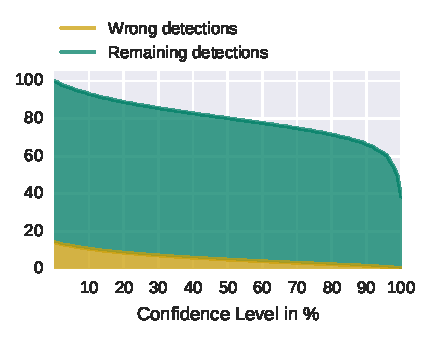
\includegraphics[width=\textwidth]{Figures/detectionsWrongConf}
        \caption[Detections]{Detections}
        \label{fig:detections}
    \end{subfigure}%
    \begin{subfigure}[b]{0.5\textwidth}
        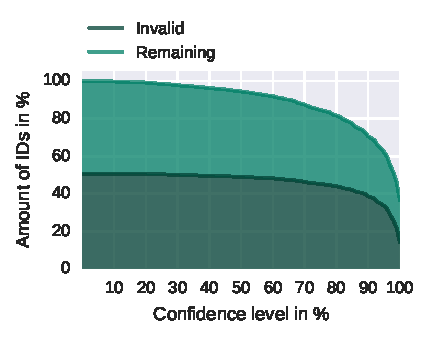
\includegraphics[width=\textwidth]{Figures/idsWrongConf}
        \caption[IDs]{IDs}
        \label{fig:ids}
    \end{subfigure}
 	\caption[Quality of detections and IDs]{\textbf{Quality of detections and IDs} \emph{Light green} represents the number of remaining data and \emph{dark green} indicates the fraction of invalid data. (a) Proportion of remaining and invalid detections. (b) IDs, that are detected at least once, in relation to invalid IDs.
 	[Data: 26.07.2016, 4~p.~m., 10~minutes, four cameras]}
 	\label{fig:remainingVSquality}
\end{figure}

\footnotetext{}

Twelve bits can encode the identity of 4096 bees.
Each bit of the decoded ID represents a probability between $0$ and $255$, normalized to a value between $0$ and $1$.
Therefore, a bit indicates the confidence of the image analysis pipeline for that specific bit.
I define the confidence $c$ for a bit $b$, analogously to Leon~\textcite[p.~14]{leon2016}, as
\begin{equation}
\label{eq:confidence}
c(b)=2\cdot|b-0.5|
\end{equation}

The confidence of a decoded ID is, accordingly, the minimum of all twelve bits' confidences.
Detections with a confidence below a certain level are removed from the data set.
Consequently, a high level of confidence reduces the amount of data available for further processing.

I use the age of the bees to check the quality of the remaining data.
If the pipeline detected a code that has not been assigned a bee will have a negative age value.
A bee has a negative age, if the pipeline detected a code, that was not used yet.
I examined the number of remaining bee detections and IDs, depending on the chosen confidence by calculating the age of each bee detection and ID.
A bee detection with a negative age is counted as an \emph{invalid detection} and an ID with a negative age is counted as an \emph{invalid ID}.

As expected, with increasing confidence levels, the number of remaining detections and IDs decreases (Figure~\ref{fig:remainingVSquality}), as does the fraction of invalid detections and IDs.
With a confidence level of 100\%, the fraction of invalid detections reaches 2.5\%.
However, the fraction of invalid IDs detected during a time interval of ten minutes remains at the high value of 30.2\%. Consequently, selecting a high level of confidence is not sufficient.
To obtain a more reliable dataset, invalid detections need to be filtered out.


%%%%%%%%%%%%%%%%%%%%%%%%%%%%%%%%%%%%%%%%%%%%%%%%%%%%%%%%%%%%%%%%%%%%%%%%%%%%%%%
%%%%%%%%%%%%%%%%%%%%%%%%%%%%%%%%%%%%%%%%%%%%%%%%%%%%%%%%%%%%%%%%%%%%%%%%%%%%%%%
\subsection{Detection Frequency Filter}
\label{subsubsec:dataset:filter}
%%%%%%%%%%%%%%%%%%%%%%%%%%%%%%%%%%%%%%%%%%%%%%%%%%%%%%%%%%%%%%%%%%%%%%%%%%%%%%%
%%%%%%%%%%%%%%%%%%%%%%%%%%%%%%%%%%%%%%%%%%%%%%%%%%%%%%%%%%%%%%%%%%%%%%%%%%%%%%%

A good indicator if a bee detection represents a real bee on the comb is the detection frequency of its ID.
Individuals with a very low detection rate may be detection errors.
To check this hypothesis, I investigate the correlation between the detection frequency of bees and their age.
Figure~\ref{fig:filter} shows that bees with a negative age are
observed less often than bees with a positive age.

During my analysis, I noticed the existence of a group of bees with a negative age and a high detection frequency.
I inspected the corresponding photos and confirmed that those bee detections correspond to living individuals and are not artifacts.
This results likely from a mistake in the reported hatching date for each bee.
Consequently, these bess were excluded from the analysis. Also I excluded bees~($n=10$), whose age is unknown\footnote{id= [2,
    74,
    2045,
    3172,
    3764,
    3796,
    3827,
    3836,
    3844,
    3940]}.

For each analysis day, the number of detections per ID is calculated, excluding the mentioned IDs.
To obtain a reliable dataset, I filtered invalid detections, by discarding all detections with an ID frequency below the 99th percentile of the negative IDs.

\begin{figure}[tp]
	\centering
	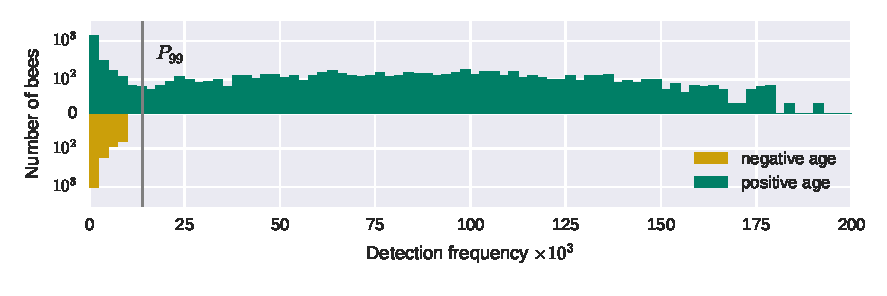
\includegraphics[width=1.0\textwidth]{Figures/filter}
	\caption[Detection frequency of IDs]{\textbf{Detection frequency of IDs} \emph{Orange} corresponds to bees with a negative age and \emph{green} displays bees with a positive age.\protect\footnotemark The \emph{gray} line represents the 99th percentile of bees with a negative age.}
	\label{fig:filter}
\end{figure}
\footnotetext{Data set: 20.08.2016, 24 hours, number of total frames: 302400}

%%%%%%%%%%%%%%%%%%%%%%%%%%%%%%%%%%%%%%%%%%%%%%%%%%%%%%%%%%%%%%%%%%%%%%%%%%%%%%%
%%%%%%%%%%%%%%%%%%%%%%%%%%%%%%%%%%%%%%%%%%%%%%%%%%%%%%%%%%%%%%%%%%%%%%%%%%%%%%%
\subsection{Time Series of Bees and Bee Pairs}
\label{subsec:tracking}
%%%%%%%%%%%%%%%%%%%%%%%%%%%%%%%%%%%%%%%%%%%%%%%%%%%%%%%%%%%%%%%%%%%%%%%%%%%%%%%
%%%%%%%%%%%%%%%%%%%%%%%%%%%%%%%%%%%%%%%%%%%%%%%%%%%%%%%%%%%%%%%%%%%%%%%%%%%%%%%
I investigated the quality of the initial data regarding its completeness of bee tracks.
A bee track represents the movement of an individual over time.
I transformed the initial data set into binary \emph{bee time series}, depicted in Figure~\ref{fig:structure} left and middle.
A bee time series, similar to a track, represents the absence and presence of a bee over a specified sequence of frames.
For further processing I use the bee time series to extract \emph{pair time series} of bees that are spatially close (Figure~\ref{fig:structure}, right).
A one indicates that a pair of bees is detected and both bees are spatially close in a certain frame.

By analyzing the resulting pair time series, I noticed that detection sequences were often interrupted by short intervals without valid detections.
As stated before, the higher the level of confidence, the more data is discarded.
This data reduction leads to more zeroes (gaps) in both time series.
Gaps in the pair time series frequently correspond to gaps in one or both bee time series and are thus the result of missing detections of the required confidence and do not represent any meaningful behavior of the bees.
Bees are not able to approach each other and move apart within a second because they simply do not move that fast.
Therefore, I concluded, that those gaps originate from detection errors and consequently need to be treated in an appropriate way during further data processing.

\begin{figure}[tp]
	\centering
	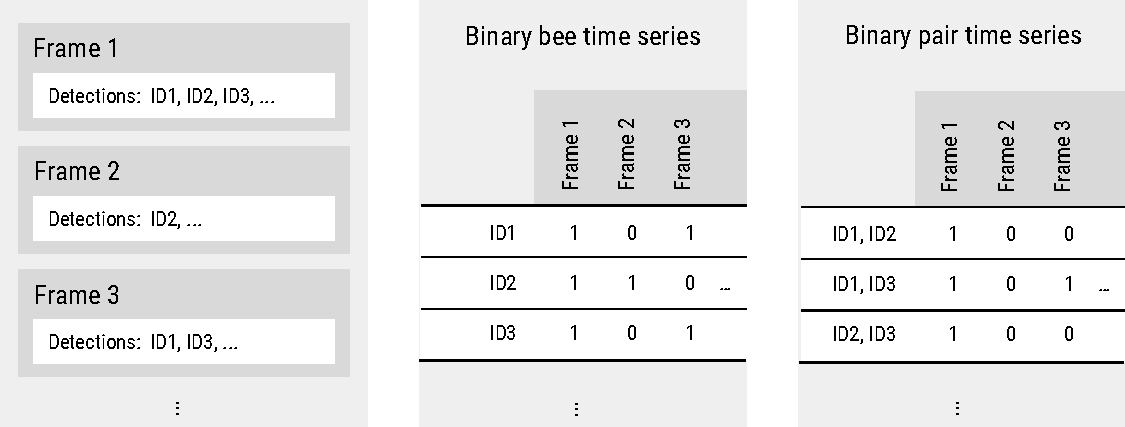
\includegraphics[width=1.0\textwidth]{Figures/structure}
	\caption[Structure of dataset]{\textbf{Structure of dataset} \emph{Left}: original dataset - containing a sequence of frames with bee detections; \emph{Middle:} binary bee time series - zero and one indicate absence and presence of a bee; \emph{Right:} binary pairs time series - zero and one indicate the absence and presence of two bees in the same frame.}
	\label{fig:structure}
\end{figure}